%!TEX ROOT = thesis.tex
\chapter{Theoretical Framework}
\section{Introduction}
In this chapter, the basic idea of ANNs is explained along with the basic functions. The keys elements of ANNs are discussed in details. It is also explained different types of network models which can be constructed by using ANNs. The parameters which are essential in the training process of the ANNs models are also described. The advantages and disadvantages of the ANNs methods are also explored further in this chapter. Moreover, it is also explained about the ANNs methods in time series forecasting in the financial market, especially in the forecasting exchanges rates. 

\section{Forecasting}
Forecasting is the process in which the future values is predicted based on the past behaviors of values of the data. Time series forecasting is one of the forecasting techniques. In time series forecasting, there are statistical methods or linear methods, and non-linear methods or ANNs. This project is proposed to use non-linear methods  time series forecasting.
\subsection{Time Series Forecasting with ANNs}

Time series forecasting involves using the available data and using it to predict the future values of this series. Forecasting exchange rates can be considered as time series forecasting. In the project,  the forecasting  is made by using ensemble ANNs model or network.

In time series forecasting, there are two types of forecasting methods which can apply. They are the single-step prediction and iterated single-step prediction or  multi-step prediction. For single-step prediction, the network is trained with several hundred of data vectors each consisting of such four days data, along with a fifth one which is the target. When the network is trained, a vector for observations of four days are supplied, and the network produces an output for the fifth day. 

Multi-step prediction is used when a long-term prediction is required. In multi-step prediction, the predicted output is fed back as input for the next forecasting and all other input units are shifted back one unit. Hence, the inputs consist of predicted values as well the original  time series data.

\section{Artificial Neural Network}
\subsection{Neurons}

A biological neuron consists of an axon, synapse, and dendrite. The inputs in biological  neuron come along by dendrite to the synapses,and when it reaches  the certain value or threshold, in other words, it fires,  and the outputs are transmitted  to another neuron. Each neuron in the brain receives several inputs and produce  an output. The inputs  are summed up to give the total input to the unit. Based on the biological neuron, the functions of a single neuron can be summarized by \citeA{beale:1990} as:
\begin{itemize}
	\item The output from a neuron is either on or off.
	\item The output depends only on the inputs, and it  needs to reach a certain number in order to make the neuron fire.
\end{itemize}

An artificial neuron constructs based on the basic functions of  a biological brain. In order to reach the limit or threshold,  the weights are added in construction the artificial neurons. After summation of inputs and weights, the results  to the  transfer functions . This artificial neuron model was proposed by McColloch and Pitts. In their model, threshold activation function was applied.

Due to its non-linear properties, a single layer neural network applies non-linearized  approach transfer function. 
\begin{figure}[hbt!]\centering
	\begin{tikzpicture}[
	init/.style={
		draw,
		circle,
		inner sep=2pt,
		font=\Huge,
		join = by -latex
	},
	squa/.style={
		draw,
		inner sep=2pt,
		font=\Large,
		join = by -latex
	},
	start chain=2,node distance=13mm
	]
	\node[on chain=2] 
	(x2) {$x_2$};
	\node[on chain=2,join=by o-latex] 
	{$w_2$};
	\node[on chain=2,init] (sigma) 
	{$\displaystyle\Sigma$};
	\node[on chain=2,squa,label=above:{\parbox{2cm}{\centering Activate \\ function}}]   
	{$f$};
	\node[on chain=2,label=above:Output,join=by -latex] 
	{$y$};
	\begin{scope}[start chain=1]
	\node[on chain=1] at (0,1.5cm) 
	(x1) {$x_1$};
	\node[on chain=1,join=by o-latex] 
	(w1) {$w_1$};
	\end{scope}
	\begin{scope}[start chain=3]
	\node[on chain=3] at (0,-1.5cm) 
	(x3) {$x_3$};
	\node[on chain=3,label=below:Weights,join=by o-latex] 
	(w3) {$w_3$};
	\end{scope}
	\node[label=above:\parbox{2cm}{\centering Bias \\ $b$}] at (sigma|-w1) (b) {};
	
	\draw[-latex] (w1) -- (sigma);
	\draw[-latex] (w3) -- (sigma);
	\draw[o-latex] (b) -- (sigma);
	
	\draw[decorate,decoration={brace,mirror}] (x1.north west) -- node[left=10pt] {Inputs} (x3.south west);
	\end{tikzpicture}
	\caption{A single layer neural network}
\end{figure}    
\subsection{Transfer Functions}
The result from summation is processed by  transfer function to produce the output.  Many other functions used are linear, threshold, gaussian, sigmoid and hyperbolic tangent functions. Due to its nonlinearity nature of the data, neural networks are constructed using non-linear transfer functions.

The sigmoid function is often used as the transfer function. In order to facilitate non-linearly of the neural network, the sigmoid function is applied. The nonlinear behavior is useful in learning since it can be more flexible in fitting curves and conditions.The mathematical and graphical representation are showed in below.
\begin{equation*}
	f(x)= \frac {1}{(1 + \mathrm{e}^{-x})}
\end{equation*}
where \\
$x$ - the inputs
\begin{figure}[hbt!]\centering
	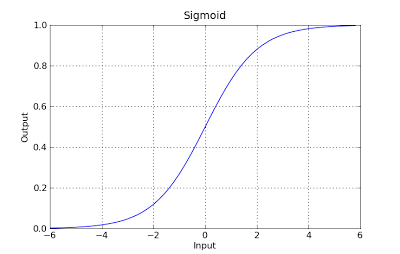
\includegraphics[width=.6\textwidth]{sigmoid}
	\caption{Sigmoid function}
\end{figure}

The sigmoid function has several properties which can be considered as one of transfer functions for this project:
\begin{itemize}
	\item The sigmoid function is inherently non-linear. This can be seen both from the graph and from the equation. Similar changes in inputs do not always produce similar changes in outputs.
	\item The sigmoid is smooth. Since the function is smooth at all points, small
	changes in inputs do not result in abrupt changes in outputs.
	\item The sigmoid function is bounded between 1 and 0. A bounded function
	introduces uniformity in processing. This is also convenient when the
	output of a neuron is used as input for the next layer. This is advantageous since the effects of extreme values are filtered out.
\end{itemize}
\subsection{Learning Paradigms}

The two learning paradigms for the neural network  are supervised and unsupervised learning.

In the supervised learning paradigm, the correct or right answers are given to the network. This type of approach  has the  knowledge of targeted outputs or desired results. It is given by many examples of the problem to train. The neural network tires and generalizes the underlying rules of the problem  during the training process. In this approach, the neural network is given a problem, to make a forecasting. This forecasting is then compared to the desired output or correct outputs which are given to the network during the training process. The learning algorithm utilizes the error information to correct the weights of  the neural network so that the next time the forecasting will be closer to the correct answer. Since the neural network learns by looking at examples, the number of examples provided has to be large enough for effective training. 

In the unsupervised learning paradigm, the neural network is asked to figure things out for itself. Unlike the supervised learning, it is not given the correct answers. The network only given the inputs data.  The task of the neural network is to look at the patterns of data and to cluster them so that similar patterns get put in the same cluster. Self-organizing networks are one of the categories of unsupervised learning because they don't have the knowledge about the desired or correct output should be. 

This project  is based on supervised learning paradigm. The neural network is supplied historical exchange rates and learns to recognize patterns from these inputs. Since the neural network knows the output of the data set, the training continues until the network is able to match the data with sufficient accuracy.

\subsection{Learning Algorithms}
Many learning algorithms have applied to train the neural network. The common algorithms are Hebb’s Rule, Gradient Descent Rule,  the Delta Rule, and back-propagation. Hebb’s Rule  is one of the earliest learning rules used in neural networks. It states that  if a processing element receives an input from another processing element, and if both are highly active, the weight between the processing elements should be strengthened.

Gradient Descent Rule used the approach of  minimizing the error between actual and desired outputs. The weights are adjusted by an amount proportional to the first derivative o f the error with respect to the weight. Though this rule is commonly used, it converges to a point of stability very slowly. The Delta Rule is also referred to as the Widrow-Hoff Learning Rule. It is also called the Least Mean Square(LMS) learning rule since it minimizes the mean squared error.

Back-propagation learning algorithm is the most commonly used generalization of the Delta Rule \cite{widrow:1990}. In the back propagation learning algorithm, the inputs are given to the network  in the input layer. The results from each layer are propagated through final layer or output layer. After it reaches the output layer, the results are compared with the given desired outputs, and   an error signal is generated.
The generated errors are propagated  back into the neural network.Each hidden layer takes into account the contributions towards the error. Based on the errors, the adjustments on weights are being computed and propagated forward to the network again.


\subsection{Types of ANNs Model}

There are many types of neural networks constructed by interconnecting neural different ways. A typical neural network consists of three layers - an input layer, one or more hidden layers, and the output layer. The input layer is the layer where the given data for things to be learned are fed. In this project, exchange rates are supplied in the input layer. The hidden layers are present to increase the total number of connections in the network, and its learning ability.Under the supervised learning paradigm, there are two popular neural network topologies which are feedforward network topology and recurrent neural networks. A network is be considered  as feedforward if it does not contain directed cycles, and is classified as recurrent if it does contain such directed cycles.

\begin{figure}[hbt!]\centering
	\begin{tikzpicture}[
	plain/.style={
		draw=none,
		fill=none,
	},
	net/.style={
		matrix of nodes,
		nodes={
			draw,
			circle,
			inner sep=10pt
		},
		nodes in empty cells,
		column sep=2cm,
		row sep=-9pt
	},
	>=latex
	]
	\matrix[net] (mat)
	{
		|[plain]| \parbox{1.3cm}{\centering Input\\layer} & |[plain]| \parbox{1.3cm}{\centering Hidden\\layer} & |[plain]| \parbox{1.3cm}{\centering Output\\layer} \\
		& |[plain]| \\
		|[plain]| & \\
		& |[plain]| \\
		|[plain]| & |[plain]| \\
		& & \\
		|[plain]| & |[plain]| \\
		& |[plain]| \\
		|[plain]| & \\
		& |[plain]| \\
	};
	\foreach \ai [count=\mi ]in {2,4,...,10}
	\draw[<-] (mat-\ai-1) -- node[above] {Input \mi} +(-2cm,0);
	\foreach \ai in {2,4,...,10}
	{\foreach \aii in {3,6,9}
		\draw[->] (mat-\ai-1) -- (mat-\aii-2);
	}
	\foreach \ai in {3,6,9}
	\draw[->] (mat-\ai-2) -- (mat-6-3);
	\draw[->] (mat-6-3) -- node[above] {Ouput} +(2cm,0);
	\end{tikzpicture}
	\caption{Typical feedforward neural network}
\end{figure}

Multilayer Perceptions (MLPs) is one to the popular neural network applied by many researchers\cite{pacelli:2011}. It is also a type of the feedforward neural network topology. In the feedforward neural networks, the expected outputs are obtained by flowing the inputs  towards the outputs layer by passing through hidden layer. In order to get the desired output, the weights in each layer are being adjusted. A typical feedforward neural network is shown in  figure 3.3 below. 

\begin{figure}[hbt!]\centering
	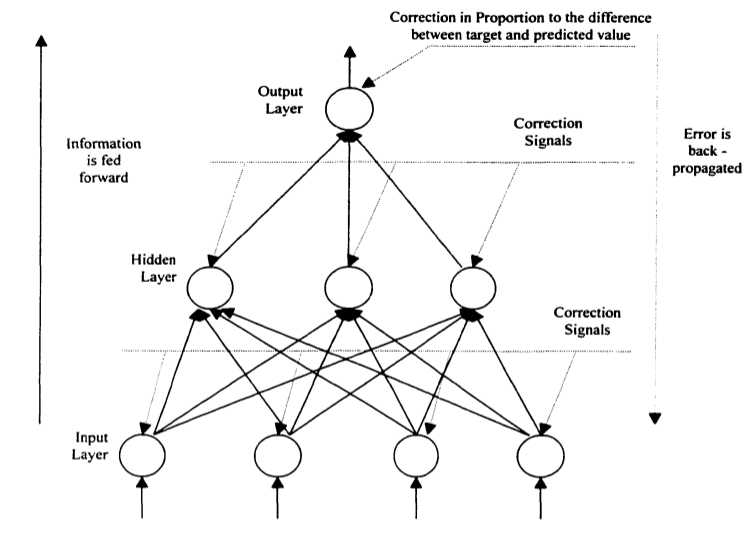
\includegraphics[width=.6\textwidth]{mlpwithBP}
	\caption{MLPs with Backpropagation}
\end{figure}

Radial basis functions (RBF) neural network is one of the methods which constructed using ANNs. This types of network are similar to MLPs, however, the function which  applied is a linear function. The main difference between traditional MLPs and RBF is that RBF is usually constructed using gaussian activation function. 

The mathematical equation for the Gaussian Activation function is mentioned below:
\begin{equation*}
	\phi(v_i) = \exp(\frac{-|| v_i - c_i ||^2}{2 \sigma^2})
\end{equation*}

where $c_i$ is the vector expressed the function center and $a$ and $\sigma$ are parameters moving the spread of the radius.

Recurrent neural networks (RNN) differ from the above configurations by the ways in which the neurons connect back to the earlier layers. The most studied and popular recurrent neural network is Hopfield network which is constructed by John Hopfield. In Hopfield network, every unit is connected to every other unit. The weights in Hopfield are symmetrical.

A graphical representation of a typical RNN is shown in figure 3.4 below.
\begin{figure}[hbt!]\centering
	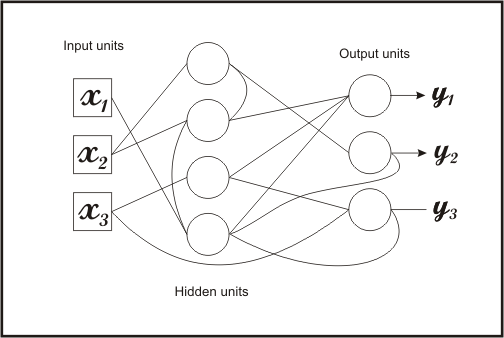
\includegraphics[width=.5\textwidth]{rnn}
	\caption{Typical recurrent neural network}
\end{figure}

\pagebreak
\subsection{Advantages and Disadvantages of ANNs}

\citeA{vellido:1999} listed some of advantages and disadvantages in their survey. As for the advantages, they mentioned;hidden nodes, in supervised ANNs models, can be regarded as latent variables,and ANNs performance can be highly automated, minimizing human involvement. As for disadvantages, ANNs are totally dependent on the quality and amount of data available, and ANNs techniques are still rapidly evolving and they are not yet robust.

Moreover, The following table explains the main advantages and disadvantages of ANNs in general \cite{lisboa:2000}. Table 3.1 is organized  in order and with the most frequent in the top row.
\begin{table}[h!]
	\centering
	\begin{tabular}{ |p{6cm}|p{6cm}|}
		\hline
		\multicolumn {2}{|c|}{\textbf{Advantages and Disadvantages of ANNs}} \\
		\hline
		\textbf{Advantages}  & \textbf{Disadvantages} \\
		\hline
		\textbf{High Accuracy:} ANNs is able to approximate non-linear mappings. & \textbf{Poor Transparency:} ANNs operates as "Black boxes". \\
		\hline
		\textbf{Independence from prior assumptions:} it do not make a priori assumptions about the data. & \textbf{Trial-error design:} the selection of hidden nodes and training parameters is heuristic.  \\
		\hline
		\textbf{Noise tolerance:} ANNs is very flexible with respect to incomplete, missing and noisy data. & \textbf{Data hungry:} it requires large amounts of data. \\
		\hline
		\textbf{Ease of maintenance:} ANNs models can be updated with fresh data, making them useful for dynamic environments.   &  \textbf{Over-fitting:} if too many weights are used, ANNs become useless for generalization to new data \\
		\hline
		ANNs overcome some limitations of other statistical methods, while generalizing them & There is no explicit set of rules to select the most suitable ANNs algorithm  \\
		\hline
	\end{tabular}
	\caption{Main advantages and disadvantages of ANNs}
\end{table}

\pagebreak

\section{Conclusion}
ANNs methods are inspired by the biological human brain. It has been many studied followed to mimic the functions of the brain. ANNs methods have the ability to learn and generalize. Many different networks are constructed using ANNs network. ANNs methods are applicable to applied in the time series forecasting. Therefore, this project is proposed to applied ANNs methods in forecasting exchange rates between Malaysian Ringgit and other currencies.